% Options for packages loaded elsewhere
\PassOptionsToPackage{unicode}{hyperref}
\PassOptionsToPackage{hyphens}{url}
%
\documentclass[
  12pt,
]{article}
\usepackage{amsmath,amssymb}
\usepackage{lmodern}
\usepackage{ifxetex,ifluatex}
\ifnum 0\ifxetex 1\fi\ifluatex 1\fi=0 % if pdftex
  \usepackage[T1]{fontenc}
  \usepackage[utf8]{inputenc}
  \usepackage{textcomp} % provide euro and other symbols
\else % if luatex or xetex
  \usepackage{unicode-math}
  \defaultfontfeatures{Scale=MatchLowercase}
  \defaultfontfeatures[\rmfamily]{Ligatures=TeX,Scale=1}
\fi
% Use upquote if available, for straight quotes in verbatim environments
\IfFileExists{upquote.sty}{\usepackage{upquote}}{}
\IfFileExists{microtype.sty}{% use microtype if available
  \usepackage[]{microtype}
  \UseMicrotypeSet[protrusion]{basicmath} % disable protrusion for tt fonts
}{}
\makeatletter
\@ifundefined{KOMAClassName}{% if non-KOMA class
  \IfFileExists{parskip.sty}{%
    \usepackage{parskip}
  }{% else
    \setlength{\parindent}{0pt}
    \setlength{\parskip}{6pt plus 2pt minus 1pt}}
}{% if KOMA class
  \KOMAoptions{parskip=half}}
\makeatother
\usepackage{xcolor}
\IfFileExists{xurl.sty}{\usepackage{xurl}}{} % add URL line breaks if available
\IfFileExists{bookmark.sty}{\usepackage{bookmark}}{\usepackage{hyperref}}
\hypersetup{
  pdfauthor={Arya Budi},
  hidelinks,
  pdfcreator={LaTeX via pandoc}}
\urlstyle{same} % disable monospaced font for URLs
\usepackage[left=3cm,right=3cm,top=2cm,bottom=2cm]{geometry}
\usepackage{graphicx}
\makeatletter
\def\maxwidth{\ifdim\Gin@nat@width>\linewidth\linewidth\else\Gin@nat@width\fi}
\def\maxheight{\ifdim\Gin@nat@height>\textheight\textheight\else\Gin@nat@height\fi}
\makeatother
% Scale images if necessary, so that they will not overflow the page
% margins by default, and it is still possible to overwrite the defaults
% using explicit options in \includegraphics[width, height, ...]{}
\setkeys{Gin}{width=\maxwidth,height=\maxheight,keepaspectratio}
% Set default figure placement to htbp
\makeatletter
\def\fps@figure{htbp}
\makeatother
\setlength{\emergencystretch}{3em} % prevent overfull lines
\providecommand{\tightlist}{%
  \setlength{\itemsep}{0pt}\setlength{\parskip}{0pt}}
\setcounter{secnumdepth}{5}
\usepackage{setspace}\singlespacing
\usepackage{pdflscape}
\newcommand{\blandscape}{\begin{landscape}}
\newcommand{\elandscape}{\end{landscape}}
\usepackage{booktabs}
\usepackage{longtable}
\usepackage{array}
\usepackage{multirow}
\usepackage{wrapfig}
\usepackage{float}
\usepackage{colortbl}
\usepackage{pdflscape}
\usepackage{tabu}
\usepackage{threeparttable}
\usepackage{threeparttablex}
\usepackage[normalem]{ulem}
\usepackage{makecell}
\usepackage{xcolor}
\ifluatex
  \usepackage{selnolig}  % disable illegal ligatures
\fi
\newlength{\cslhangindent}
\setlength{\cslhangindent}{1.5em}
\newlength{\csllabelwidth}
\setlength{\csllabelwidth}{3em}
\newenvironment{CSLReferences}[2] % #1 hanging-ident, #2 entry spacing
 {% don't indent paragraphs
  \setlength{\parindent}{0pt}
  % turn on hanging indent if param 1 is 1
  \ifodd #1 \everypar{\setlength{\hangindent}{\cslhangindent}}\ignorespaces\fi
  % set entry spacing
  \ifnum #2 > 0
  \setlength{\parskip}{#2\baselineskip}
  \fi
 }%
 {}
\usepackage{calc}
\newcommand{\CSLBlock}[1]{#1\hfill\break}
\newcommand{\CSLLeftMargin}[1]{\parbox[t]{\csllabelwidth}{#1}}
\newcommand{\CSLRightInline}[1]{\parbox[t]{\linewidth - \csllabelwidth}{#1}\break}
\newcommand{\CSLIndent}[1]{\hspace{\cslhangindent}#1}

\title{Contagious Turnout during Infectious Pandemic:\\
A Spatial Analysis}
\usepackage{etoolbox}
\makeatletter
\providecommand{\subtitle}[1]{% add subtitle to \maketitle
  \apptocmd{\@title}{\par {\large #1 \par}}{}{}
}
\makeatother
\subtitle{DRAFT}
\author{Arya Budi}
\date{}

\begin{document}
\maketitle

~ Election bears spatial dimension when it meets infectious pandemic.
General public suspects that the rise of infections after the election
might relate to how the election was conducted. But, how about if this
``cliche suspicion'' does not happen, i.e., electoral participation does
not contribute to the rise of Covid-19 infections. There are cases when
an election is held during a heyday of life-threatening health risks.
Still, electoral adjustments and special voting arrangements, including
early voting, postal voting, proxy voting, home voting, and polling
station arrangements, as documented by Asplund et al. (2021) and
colleagues, are absent. In a setting of a voluntary voting system, why
did some voters vote and others did not during the pandemic? While a
large number of scholarships on voter turnout address individual-level
behavior and system-level factors, does space and location matter in
explaining the turnout in a time of crisis? Thus, this paper addresses
the effect of Covid-19 on electoral participation rather than the
reverse.

~ By incorporating spatial econometrics Anselin (2007) into the model
specifications, this paper tries to uncover how location and space
affect human behavior in voter turnout. As a pilot project, this
research examines the mayoral election in Surabaya city, Indonesia, held
in December 2020. While turnout in 2015 (51\%) and 2010 (44\%) were also
relatively low, more people in 2020 (53\%) came to polling stations when
infectious viruses threatened the whole population. In a crisis, a high
percentage of electoral participation in a voluntarily voting system
seems counterintuitive.

~ Yet, the proximity of spaces and locations that approximate the extent
to which social interactions occur might explain such a political
behavior. The findings suggest that electoral participation is
``infectious,'' relative to the Covid-19 virus when elections were held
during the pandemic. This paper argues that the contagion of turnout in
such a time of crisis is arguably a result of neighboring effects. The
imitation/diffusion theory of the neighboring effect explains the
counterintuitive case in Surabaya and other places where turnout is
higher in times of crises than that in a regular election before the
pandemic.

~This paper will be delivered as follows. The first section surveys
central premises about the effects of institutional arrangement on
turnout that may and may not work in a time of the pandemic. The
following section provides some possible models that arguably work for
turnout theory. Third, I propose the spatial approach of turnout that
may explain an increase in turnout during the pandemic. Then, I
elaborate on the data and method outlining my empirical strategy on
spatial econometrics. Lastly, I report the results, followed by a
discussion.

\hypertarget{institutional-arrangement-and-turnout}{%
\section{Institutional Arrangement and
Turnout}\label{institutional-arrangement-and-turnout}}

~ Literature on voter turnout suggests several drivers and perspectives
that explain the macro and microfoundation of voter turnout. At the
macro-level theories, system-level variables and institutionalist's
points of view are the central premises. Some models of the micro-level
models, including scholarships from utility maximization of a rational
actor and political mobilization models, are linked to the macro-level
variables. Other individual-level models, such as habitual,
motivational, and citizen-duty variables (see Cebula, Durden, and Gaynor
2008; Aldrich, Montgomery, and Wood 2011; Dinas 2017), obviously explain
voter turnout but they are not directly connected with the effect of
institutional arrangements.

~ Institutional arrangement and administration are some of the other
oceanic literature on turnout. As the ``big picture of electoral
turnout'' (Vowles (2017)), many authors in this area suggest that
electoral system affect turnout where proportional representation
electoral system (hereafter, PR system) (Bormann and Golder 2013) and
compulsory voting (Blais 2000; Franklin 1999; Geys 2006). Geys (2006)
argue that the effect of compulsory voting on turnout is one of the
robust findings. A meta-analysis by Stockemer (2017, 705) nevertheless
finds that some studies do not support the positive relationship of PR
system. Yet, proponents of the PR effect argue that districts are more
competitive due to the nature of multimember districts. Large campaigns
and political mobilization from a large number of the candidates
increase turnout (for initial study, see Blais and Carty 1990).

~ However, such system-level variables are impossible to adjustment in a
crisis. Instead, administrative arrangements are plausible in a time of
crisis. In this regard, we deal with electoral management and
administration of voting and polling station as the driver of turnout.
Comparative electoral administration addresses a voting engineering
mainly in the forms of voting by mail and early or absentee ballot
voting. For instance, Gerber, Huber, and Hill (2013) provide evidence
that all-mail elections improve turnout by about 2-4 percentage points.
Gronke and Miller (2012) even find that the increase of turnout by mail
is about ten percentage points (for a similar case, see also Richey
2008; Southwell and Burchett 2000; Karp and Banducci 2000).

~ Meanwhile, the distance of polling stations has been vastly examined
across elections and countries (see Cantoni 2020; Dyck and Gimpel 2005).
Others find that accessibility and location of polling stations also
convey a significant relationship (Schur, Ameri, and Adya 2017; Brady
and McNulty 2011; Orford et al. 2011). The significant association of
distance and location of the polling station with turnout suggests that
the spatial dimension of electoral management matters in turnout.

~ These studies, nevertheless, do not address how such administrative
arrangements of voting and polling sites operate in the context of
pandemics or crises. Furthermore, some studies have documented the
adverse effects of Covid-19 on turnout (see, for instance, Haute et al.
2021; Noury et al. 2021; Nwankwo 2021). Nonetheless, they are not
sensitive to how electoral administrative arrangements and electoral
politics intersect with the nature of infectious pandemics where
geographical proximity of the virus affects political participation.
Moreover, studies investigating the effect of the institutional
properties of election during the pandemic (see Pettigrew 2021),
especially polling sites, do not specify spatial components (measures
and parameters) into their model specification.

\hypertarget{turnout-in-a-time-of-crisis}{%
\section{Turnout in A Time of
Crisis}\label{turnout-in-a-time-of-crisis}}

~ In a crisis, electoral adjustment is only feasible when it is
politically and logistically gratuitous. Changing electoral systems and
the related properties, such as ballot structure and electoral formula,
is politically costly as the change will directly affect the electoral
gains. Shifting an in-person ballot to other types of a distance voting,
such as e-voting and voting by mail (postal voting), can be regarded as
politically feasible. Yet, such special adjustments of voting require
extensive resources, ranging from infrastructure, staffing, security
issues and cost. An archipelagic country such as Indonesia will be
extremely difficult to address postal voting during a pandemic as a
prolonged crisis.

~ Because of the constant mode of in-person voting, electoral battle
remains on the ground during the voting day. At the same time, voters
are haunted by the Covid-19 proximity in their neighborhood by keeping
an eye how a crowd may occur in the polling sites. Thus, we have three
possible cross-sectional models that relate to voter turnout during the
pandemic: administrative adjustment, political mobilization, and
proximity of crisis.

\hypertarget{administrative-adjustment-polling-sites-population-size}{%
\subsection{Administrative Adjustment: Polling Site's Population
Size}\label{administrative-adjustment-polling-sites-population-size}}

~ Under the absence of convenient (or distance voting), engineering
polling stations by enlarging their number, so lowering the size of
voters in each polling site than usual elections, is a plausible
electoral adjustment. Though it looks simple, reducing population size
is arguably pre-empt the overcrowding of voters on election day; the
crowd is a critical issue during the infectious pandemic. Though most
studies agree with the negative effect of population size on turnout
(Geys 2006, 642), the competing debate remains in the homogeneity
thesis. They argue that a smaller size of population that generates
homogeneous society increases turnout as group solidarity and feasible
linkage between politicians (or political leaders) and voters foster
people to vote (Kostadinova and Power 2007). However, in a time of
crisis, population size relates to the extent to which voters expect
their health risk. People are cautious when overcrowded in the polling
site is expected. All these institutional arrangements and adjustments
return to the theoretical premise of the cost of voting. Drawing on this
notion, this model argues that the larger size the polling site's voter
population, the lower the turnout.

\hypertarget{proximity-of-crisis-covid-19-infections}{%
\subsection{Proximity of Crisis: Covid-19
Infections}\label{proximity-of-crisis-covid-19-infections}}

~ Following Downsian rational-choice model, the proximity of crisis
(i.e., the extent to which Covid-19 infections occur in the neighboring
area) affects political participation. This mechanism is similar to the
population size model. As pioneered by Downs (1957), rational-choice
model has been employed extensively to explain behavioral premises of
voter turnout. This model, nevertheless, is hardly ever to link with
institutional factors such as administrative arrangements of how an
election is held. It primarily suggests the idea of the cost of voting
or ``calculus of voting'' derived from the utility function from
rational-choice theory (see Aldrich and Jenke (2017)). In addition, the
role of information distribution is also under this model (Feddersen and
Pesendorfer (1999)). For instance, though Morton et al. (2015) estimate
the effect of exit poll information on the decreasing turnout, they
suggest that exit poll information also increases bandwagon voting.
Similarly, in the case of the Covid-19 pandemic, a voter is expected to
stay at home when any type of distance voting is absent, as people
hesitate when surroundings are infectious. Based on the cost of voting
related to helth risks, this model suggests that the higher the
infection, then the lower turnout.

\hypertarget{close-election-political-mobilization}{%
\subsection{Close Election: Political
mobilization}\label{close-election-political-mobilization}}

~ An election is somehow a political contest among candidates (or
parties) that situate them to compete by mobilizing voters to vote for
their electoral gain. Other than pandemic-related arguments, thus,
political mobilization model may give us an enduring theory of voter
turnout, either in normal or crisis circumstance. Political mobilization
theory relates to the idea of a close election. By close election, it
means that when there are two competing candidates who contest
competitively, indicated mostly by a small vote margin, the likelihood
the voters cast their votes is higher than an election under uncontested
candidates or non-competitive race (Cann and Cole 2011; Grofman 1995;
Indridason 2008; Simonovits 2012). Close election situates candidates to
mobilize voters and media to report more coverage regarding the
contesting candidates, which boost people to vote. Based on their
massive field experiment, Green and Gerber (2019) documented several
campaign approaches of get-out-the-vote techniques that foster turnout,
including mail, postcard, and in-person visit (canvassing) increase
turnout (Gerber and Green 2000, 2005). Though they find null finding on
phone-call, Imai (2005), based on replication of Gerber and Green's
field experiment data, maintain that phone-call does positively affect
on turnout. As a close (or competitive) election indicates the extent to
which the candidates mobilize voters, this model suggests that a
competitive electoral district has a higher turnout than that of
non-competitive electoral constituency.

~ Lastly, demographic characteristics have been crucial variables that
possibly confound those models. Demographic characteristics, such as
income and education, have always been inevitable variables in
explaining voter turnout (Plutzer 2017). For instance, a high level of
education and literacy rate is linked with electoral participation
Diwakar (2008). In short, we need to control for these variables should
we examine those three models.

\hypertarget{contagious-turnout-a-spatial-model}{%
\section{Contagious Turnout: A Spatial
Model}\label{contagious-turnout-a-spatial-model}}

~ The cross-sectional models elaborated earlier, nevertheless, are
contingent on the context where social interactions occur. Therefore I
propose an alternative theory that explains turnout beyond a time of
pandemic: contagious turnout. This theory potentially addresses a set of
questions posed earlier, based on the counterintuitive case: why turnout
in a time of crisis increases. I contend that the decision-making of
turnout is 1) a product of turnout in the neighboring areas or 2) other
unobserved variables that situate turnout decision due to the variables'
spatial dimension. In spatial econometrics (Anselin and Florax 1995;
Anselin 2007), the former mechanism refers to a spatial lag dependence
model and the latter constitutes a spatial error model; that I will
elaborate on the econometrics behind these models later. For now, I
focus on substantive premises that explain the contagious turnout.

~ As turnout is contagious, we may expect that turnout is spatially
clustered or structured, e.g., there will be a high turnout in one
geographic area and a low turnout in another region. Though the school
of thought in spatial analysis provides several mechanisms that explain
spatial patterning (see, for instance, Voss et al. 2006; Cho and Rudolph
2008), I contend that the contagious nature of turnout is more driven by
two mechanisms. . First, it is an imitation/diffusion mechanism that
emphasizes multi-directional interactions. The second mechanism relates
to an external-force mechanism that situates turnout as a response for
such forces, including political mobilization and group responses.

~ Regarding the imitation mechanism, explicit and implicit interactions
operate in electoral participation. Explicit (direct) interactions lead
to information distribution that affects turnout (Feddersen and
Pesendorfer (1999)). In terms of implicit interaction, low-intensity
interaction where political participation is a result of casual
observations of the surroundings, such as yard signs, stickers, or flags
(Cho and Rudolph 2008). In the case of turnout during pandemic, people
are prone to perceive that the risks are minimal when they see voting
goers crossing their neighborhood area. Merkley et al. (2022) suggest
that safety precautions explain in-person turnout during the pandemic.
Nevertheless, because of spatial proximity, explicit interaction (e.g.,
verbal conversation) or implicit causal observation by seeing people
come to polling sites reduces such safety precautions, driving voters
under such interactions turnout. This is why this mechanism is also
referred to as neighboring effects.

~ One may suspect that today's digital environment challenges the
spatial clustering of such political interactions due to distance
interactions. Yet, in cases where voters must attend polling sites due
to the absence of distance voting administration, information and
interactions that operate either offline or online most likely concern
the risk of attending polling sites during the infectious pandemic.
Attending polling sites resembles imitation and diffusion of neighboring
effects as people get out to vote as their neighbors do so. Once voter
turnout is spatially clustered and structured, we conclude that this
spatial effect occurs.

~ Related to the second mechanism, spatial structure of turnout can be
driven by various forces, but political forces and group response are
potential major forces. In terms of f political mobilization, candidates
will strategically target specific areas where large number indifferent
(swing) voters are expected and ``social networks may develop in
response to mobilization'' (Cho 2003, 370). Accordingly, political
interactions occurring between candidates (or the campaign team) and
potential voters potentially generate spatial structure. As an
elite-driven process of social interaction, political mobilization at
the battlegrounds where a close (competitive) election is likely to
occur is expected to drive geographical clusters of interactions (see
Rosenstone and Hansen 1993; Cho and Rudolph 2008).

~ Furthermore, the external-force mechanism is also a product of group
responses (Voss et al. 2006) and inter-group interaction (Cho and Baer
2011). At the micro-level view, individuals living in the same area
share common attributes or characteristics, such as geographical
conditions, labor practices, or industrial structures, where these
characteristics situate people to ``respond similarly to external
forces'' (Voss et al. 2006, {[}376{]}). Meanwhile, social organizations
and informal commonality at the neighborhood level may also generate a
uniform response (in an aggregate measure) in the way how people
participate in an election. Individual interactions, in turn, create a
group response at the space dimension, which produces a spatial
clustering in the context of contagious turnout.

~ Putting all these altogether, once we find a conclusive spatial
pattern of turnout, that indicates that contagious turnout operates
during the pandemic. It also means that the three cross-sectional models
may not be supportive enough to explain the rise of turnout in a time of
crisis. In order to prove whether cross-sectional or contagious theories
operate in the time of pandemic, the next section elaborates on data and
method.

\hypertarget{data-and-method}{%
\section{Data and Method}\label{data-and-method}}

\hypertarget{data}{%
\subsection{Data}\label{data}}

~ This study examines data based on Surabaya Mayoral Election,
Indonesia, held in 2020. To be sure, the election was contested by two
candidates who, to some extent, made the case suitable to examine the
models. Other than data availability and research feasibility, the
municipal administration provides Covid-19 aggregate data on a daily
basis regarding its 154 village-level units. This data juxtaposes with
mayoral-election data provided by Indonesian General Election Commission
which is also at village-level units. The third data set on demographic
characteristics (education and income), i.e., a 2000-respondent exit
poll data set from my previous project (see Budi 2021), complement the
two key datasets.\footnote{The exit poll project covers all 152 villages
  proportionally with minimal 10 respondents. Therefore, two villages
  are not covered in the exit poll project due to its very small size of
  the voter population. As my village-level aggregation of this data may
  embody a statistical artifact, I am still trying to seek village-level
  demographic profiles that might be provided by a Statistics Bureau.}

~ In addition, in the case of aggregate-level studies, a small unit of
electoral constituencies, such as the village-level unit, may uncover
such spatial patterning of social-political interactions. It is because
neighborhood politics and social interactions occur among voters at the
village level where polling sites are administered, Covid-19 infection
cases are registered and reported, and the votes are contested.

\normalsize

\begin{figure}
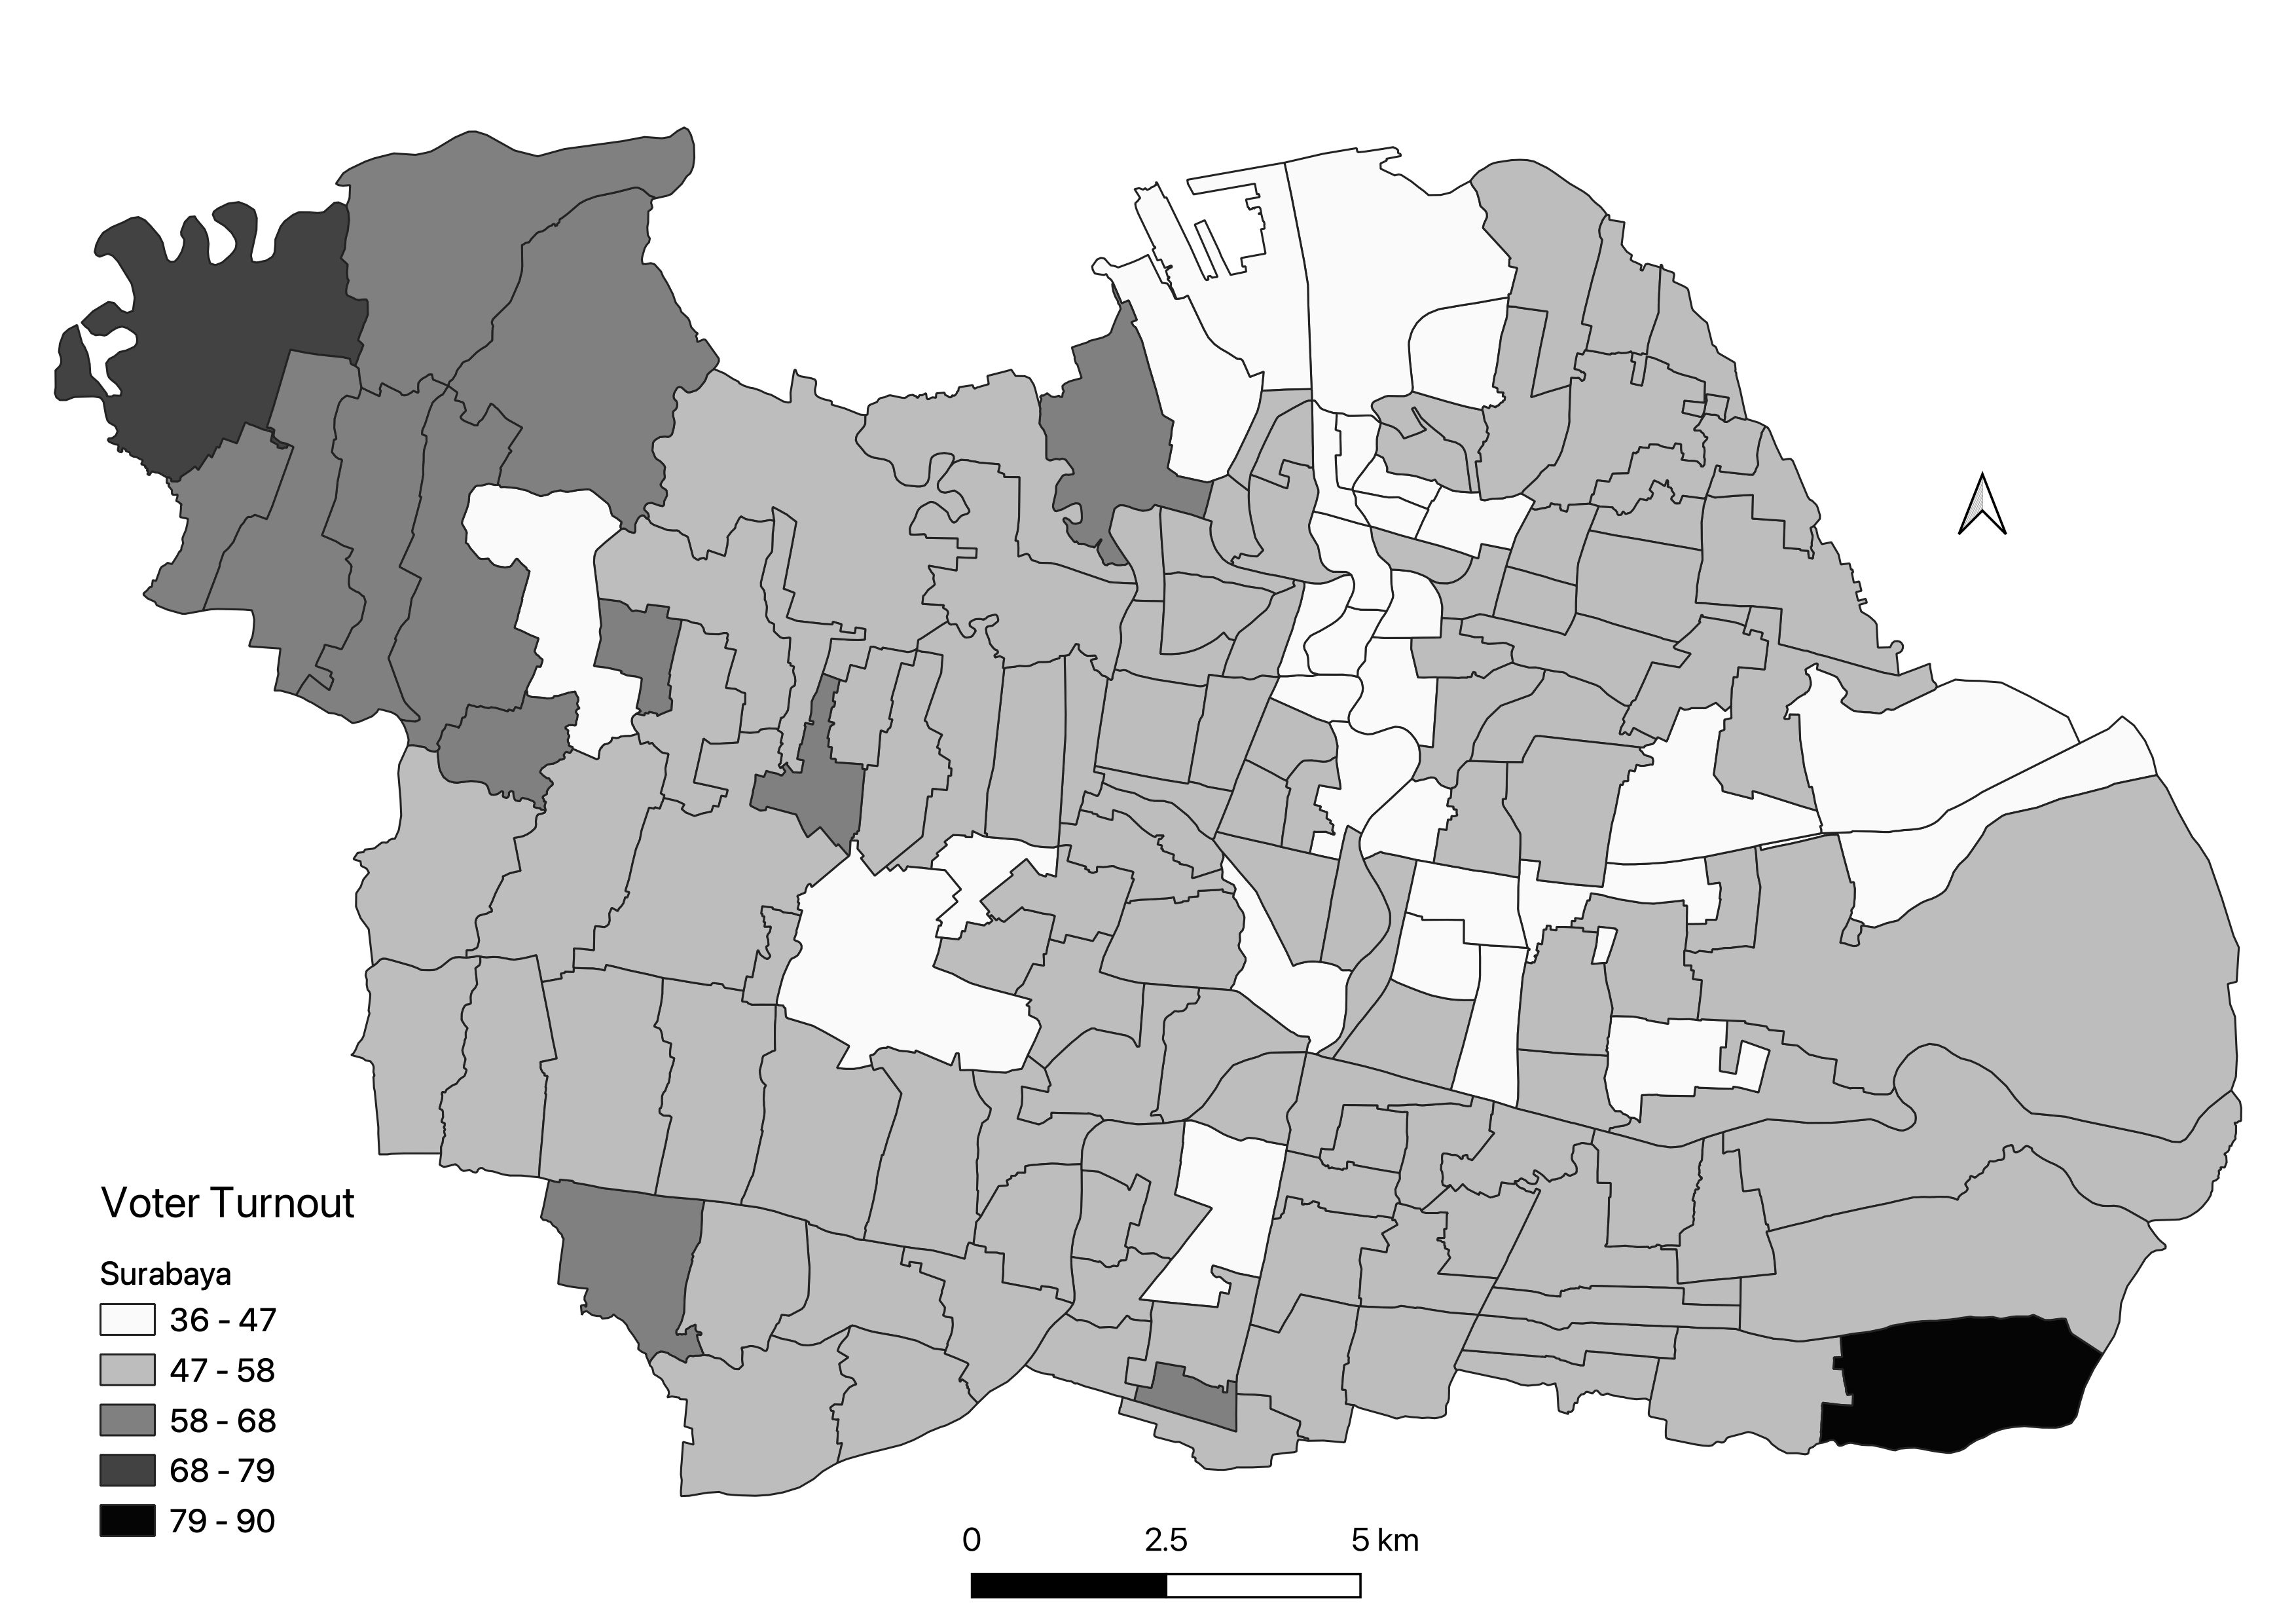
\includegraphics[width=0.48\linewidth]{DistVTO17Dec} 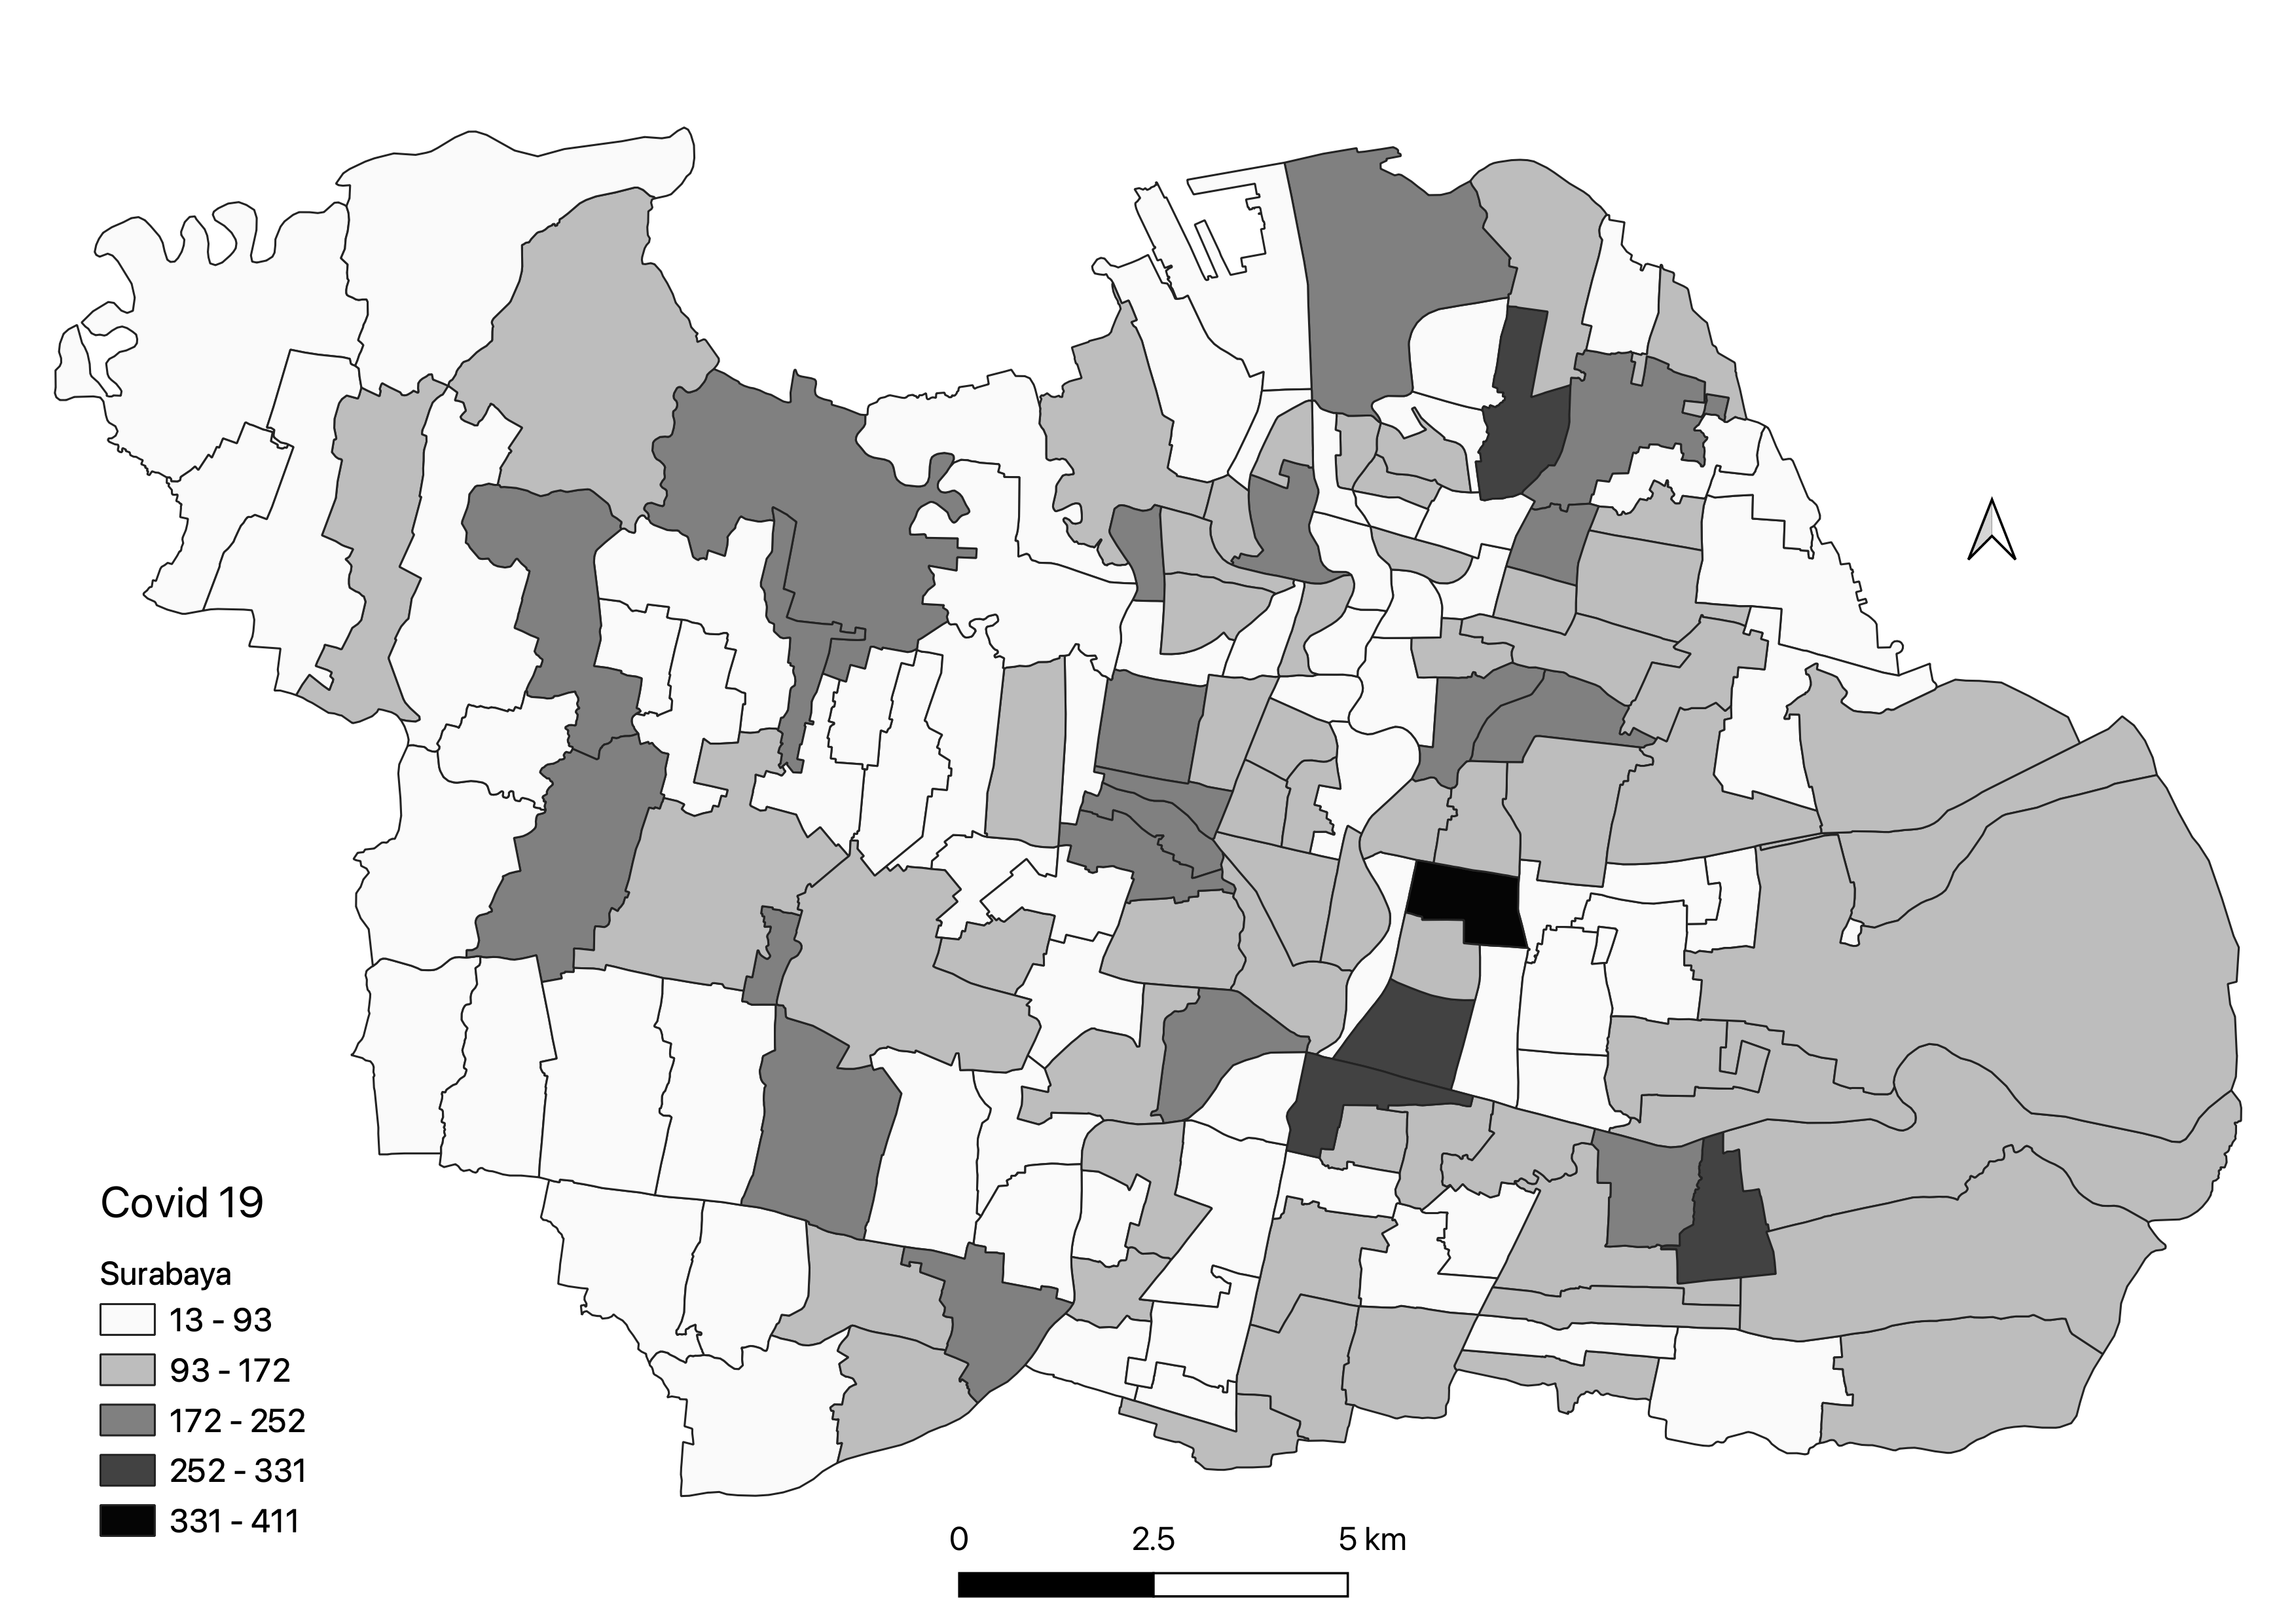
\includegraphics[width=0.48\linewidth]{DistCovidDec17} \caption{Voting during Covid-19 Pandemic in 2020 Surabaya Mayoral Election}\label{fig:desctip}
\end{figure}
\normalsize

~ Figure 1 shows the spatial distribution of Covid-19 infection cases in
the left-side map and electoral participation in the right-side map. We
see that the voter turnout is relatively high, indicated by 50\% or more
turnout, in the northwestern villages, while the distribution of
Covid-19 infection cases is also relatively low, marked by ten or more
minor cases, in the region. At a glance, these maps give us a sense that
the relationship between turnout and Covid-19 pandemic is negatively
associated. Though this interpretation is premature as we need to
investigate further the spatial models, the distribution of Covid-19 and
turnout relates to the results and analyses elaborated later.

\hypertarget{variables}{%
\subsection{Variables}\label{variables}}

~ I define voter turnout, the dependent variable, as a percentage of the
number of total votes by total registered voters. I acknowledge that
other authors employ voting age population as the denominator, rather
than the registered voters. Yet, the village-level data only provide an
official record of the registered voters. Besides, the number of the
registered voters is presumably slightly the same as that of the
voting-age population.\footnote{There is a procedure where individuals
  who are able to prove their state ID are eligible to vote even though
  they are not registered in the electoral data base. In addition, the
  Indonesian General Commission have validated their data in several
  ways before the voting day to make sure all the eligible residents are
  registered.}

~ To examine the cross-sectional models, I develop several explanatory
variables. The first explanatory variable, i.e., the average voter
population size in each polling site, deals with the number of polling
stations and the total number of voters. I expect that higher turnout
occurs in villages with smaller polling sites' population sizes. For the
political mobilization thesis, approximated by close election, the other
independent variable addresses the difference between the number of
voters gained by the two candidates. Thus, the smaller the contrast of
the votes indicates a high level of competitiveness, approximating
extensive mobilization in the given village. Lastly, the proximity of
Covid-19 refers to the rise of the infection cases one week before the
election. The rise of infection cases sets the alarm to the voters not
to take their health risk by attending polling sites. I also control for
demographic profiles, especially education and income, though this
paper's data on demographic covariates are subject to change. I report
these variables in Table 1.

\normalsize
\begin{table}[!htbp] \centering 
  \caption{Descriptive Statistics of the Variables} 
  \label{} 
\small 
\begin{tabular}{@{\extracolsep{1pt}}lccccc} 
\\[-1.8ex]\hline \\[-1.8ex] 
Statistic & \multicolumn{1}{c}{N} & \multicolumn{1}{c}{Mean} & \multicolumn{1}{c}{St. Dev.} & \multicolumn{1}{c}{Min} & \multicolumn{1}{c}{Max} \\ 
\hline \\[-1.8ex] 
Voter Turnout & 154 & 50.90 & 5.93 & 36.41 & 89.63 \\ 
Polling Site's Population Size & 154 & 402.70 & 16.00 & 339.00 & 442.50 \\ 
Covid-19 Proximity & 154 & 3.46 & 3.30 & 0 & 17 \\ 
Competitiveness & 154 & 1210.00 & 965.10 & 10 & 4607 \\ 
Income (Aggregate) & 152 & 0.26 & 0.18 & 0.00 & 0.75 \\ 
Education (Aggregate) & 152 & 0.19 & 0.18 & 0.00 & 0.88 \\ 
\hline \\[-1.8ex] 
\multicolumn{6}{l}{$*$ Obervations are village-level units} \\ 
\end{tabular} 
\end{table} 
\normalsize

\hypertarget{method}{%
\subsection{Method}\label{method}}

~ My empirical strategy heavily employs spatial econometrics (see
Anselin 1995, 2006, 2013) by addressing data on hundreds of
village-level units in Surabaya. The underlying assumption is that the
units are not independent since social interactions are inevitable.
Thus, spatial approximation, known as spatial weight matrix, is
necessary to measure the extent to which the interactions occur and
affect the resulting behavior of voter turnout. In this regard, I employ
first-order queen contiguity for the spatial weight matrix (\(W\)). The
relatively small data set of 154 villages situates this paper to apply
first-order contiguity rather than second-order contiguity. Moreover,
queen contiguity here aims to have all the surrounding village
neighbors, even those that share a small magnitude of
borderlines.\footnote{Results from rook contiguity also generates
  similar coefficient of the global Moran's I test statistics as the
  difference is about 0.001.}

~ Based on that basic logic, assessing the randomness of the
observations scattered across spaces and locations is imperative. In
many instances, the spatial patterning is a result of demographic groups
living in the nearby area (see Cho and Gimpel 2010). Autocorrelation,
computed mostly through Moran's I statistics, is a stochastic method
that gauges the spatial randomness of observations, i.e., whether the
units' variable of interest is spatially clustered/structured or random.
In other words, once we find a significant positive coefficient of the
Moran's I statistics, we may \emph{temporarily} conclude that voter
turnout is spatially correlated (clustered), i.e., a high (or low)
turnout in one village is associated with a high (or low) turnout in its
surrounding villages. Global Moran's I Statistics is computed as
follows.

\begin{align}
I = \left(\frac{n}{\sum_i \sum_j w_i{_j}} \right) \ \left(\frac{\sum_i \sum_j w_i{_j}(x_i - \mu)}
{\sum_i (x_i - \mu)^2}\right)
\end{align}

where i and j index the spatial units of which there are \(n\),
\(w_i{_j}\) is an element of a row-standardized spatial weights matrix,
\(x\) is the percent of turnout, and \(\mu\) is the average percentage
of turnout in the sample.

~ While we are equipped with the statistics to assess spatial patterning
across all the village-level units, the Local Moran's I, or local
indicators of spatial autocorrelation (LISA), are able to show the
spatial clustering of turnout between the neighboring units. This test
statistic is computed as follows.

\begin{align}
I_i = \left(\frac{z_i}{\sum_i z_i^2} \right) \ \left({ \sum_j w_i{_j} z_j} \right)
\end{align}

where \(z\) is the mean-deviated form of the percent of turnout in
particular villages.

~ Once we find a positive and significant result in the Moran's I
statistics, i.e., an indication of spatial patterning of voter turnout,
we need to specify the spatial autoregressive models. The models,
primarily investigated through spatial lag dependence or spatial error
models, estimate the spatial effects of the variable of interests or the
error relating to any omitted (unobserved) variables that are spatially
correlated on voter turnout. The spatial lag dependence model is
computed as follows.

\begin{align}
y = \rho W y \ + \ X \beta \ +  \varepsilon
\end{align}

where \(y\) is a vector that represents the dependent variable of voter
turnout, \(W\) is an n × n spatial weights matrix, \(\rho\) is the
spatial autoregressive constant to be estimated, \(X\) is the
explanatory variables with \(\beta\) as the coefficients, and
\(\varepsilon\) is the error term. Meanwhile, we seek whether there is
an error that relates to spatial attributes of any omitted variables
through the following spatial error equation.

\begin{align}
y =\ X \beta \ +  \epsilon
\end{align}

and

\begin{align}
\epsilon = \lambda W \epsilon + \varepsilon
\end{align}

where \(\lambda\) is the spatial lag parameter to be estimated and the
other terms are similar to the equation (3). As we are not sure whether
spatial lag or spatial error models explain the spatial patterning of
turnout regarding our variables of interest, Lagrange Multiplier (LM)
test statistics are employed to determine the model that generates a
significant result.

~ The spatial autocorrelation and autoregressive statistics have been
applied across disciplines that take spatial effects into account (see,
for instance, Baller and Richardson 2002; Voss et al. 2006). Given the
nature of the spatial analyses and the geospatial data, I employ a
series of data processing in R, GeoDa, and QGIS software.

\hypertarget{results}{%
\section{Results}\label{results}}

\hypertarget{contagious-turnout-a-comparison}{%
\subsection{Contagious Turnout: A
Comparison}\label{contagious-turnout-a-comparison}}

~ Figure 2 shows that the electoral participation (the left plot),
approximated by the percentage of voter turnout, is even more
``infectious'' than the virus shown on the right plot. This comparison
is not intended to test the theory I have proposed earlier. Rather, a
comparison between turnout and Covid-19 spatial autocorrelations is to
demonstrate the extent to which turnout is contagious. As displayed on
the left-hand side of Figure 2, the turnout is significantly spatially
associated (p \textless{} .05). Though the autocorrelation coefficient
\(r\) (.390) is not high, indicated when \(r>.50\), the plot clearly
shows that high turnout in one village has a link with a high turnout of
the neighboring villages, and vice versa. In other words, turnout is not
spatially random as the Moran I's statistics indicate the presence of
spatial patterning.

\normalsize\normalsize

\normalsize

\begin{figure}
\includegraphics[width=1\linewidth]{figs/figmoranplot-1} \caption{Global Moran's I Statistics of Voter Turnout Percentage and the Covid-19 Infection Cases A Week before Voting Day}\label{fig:moranplot}
\end{figure}
\normalsize

~ In contrast, the Covid-19 infections before the mayoral election are
not strongly spatially clustered with a very low autocorrelation
coefficient \(r\) (.004). In other words, infections in one village are
not strongly associated with infections in other villages. The
insignificant result of the Covid-19 cases is a surprising finding. But,
epidemiologists, including the Indonesian government, suggest that
family-based cluster of infections have massively taken place in 2020
(see Soedarsono 2020). This result of autocorrelation of the Covid-19
infections seems to confirm such claims. The spatial patterning, or
spatial clustering, becomes more evident when we see the spatial mapping
of the local Moran's statistics.

\normalsize

\begin{figure}
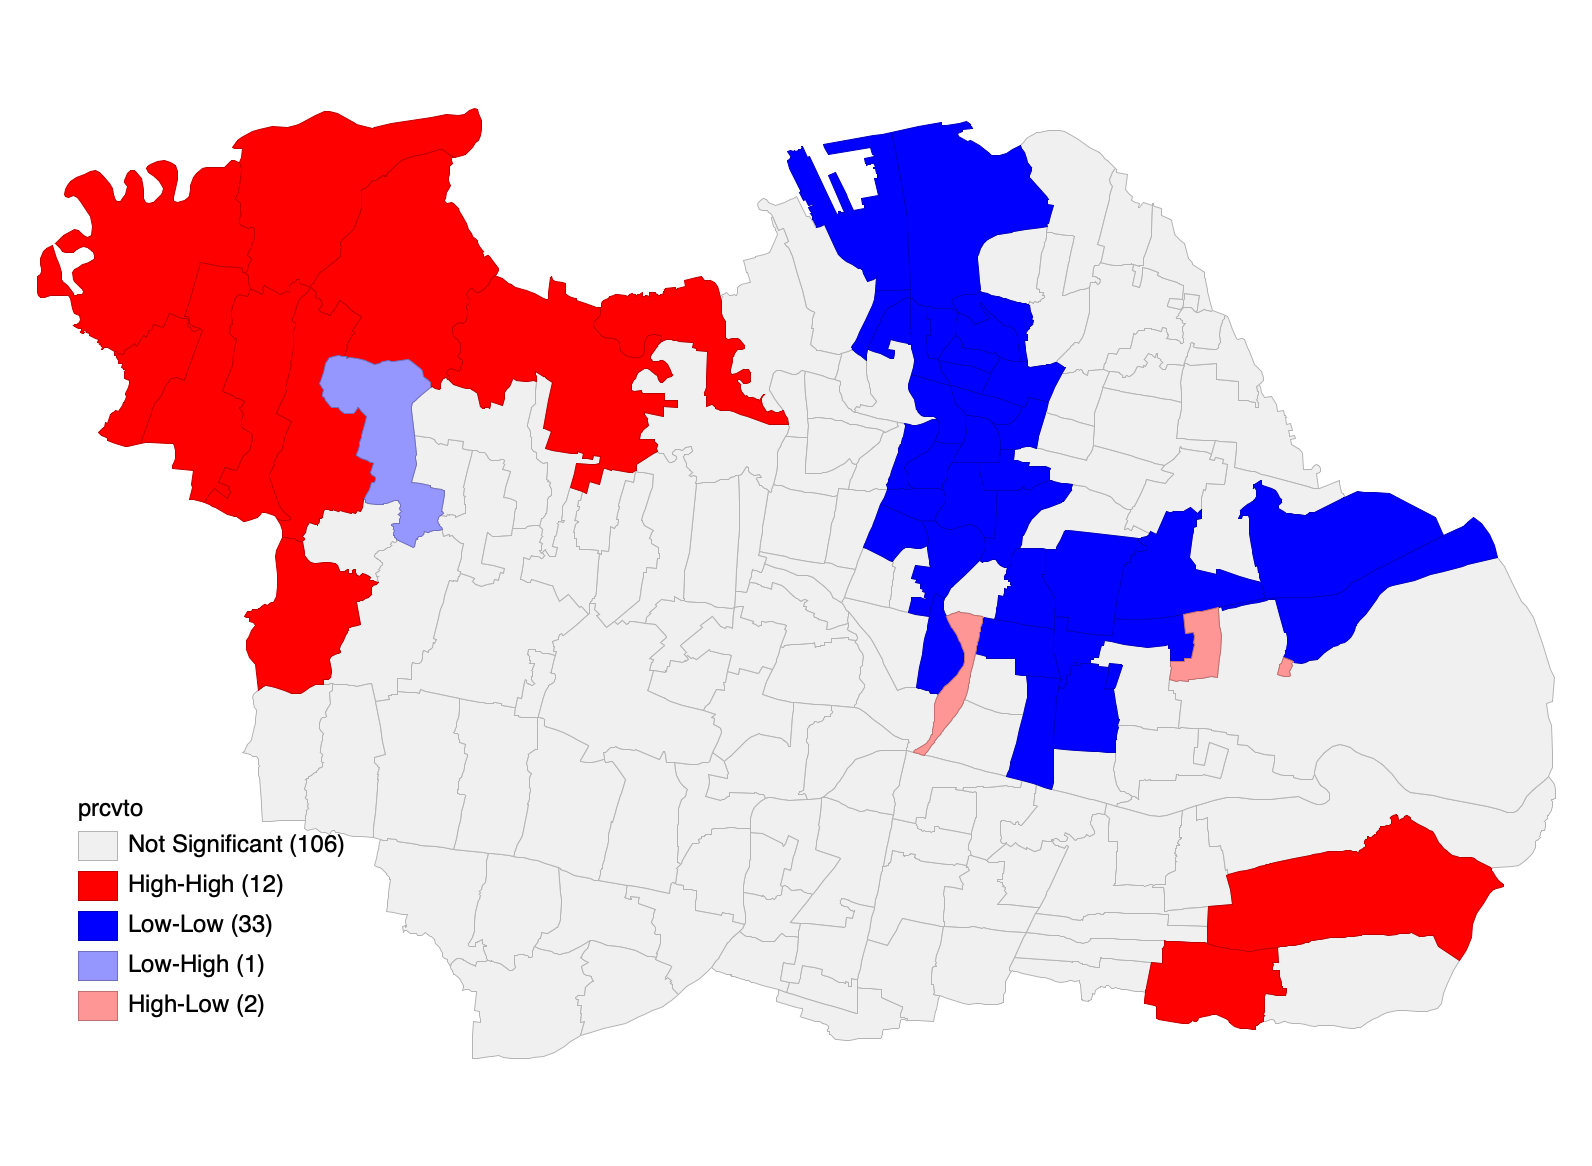
\includegraphics[width=0.49\linewidth]{LocalMoran-VTO} 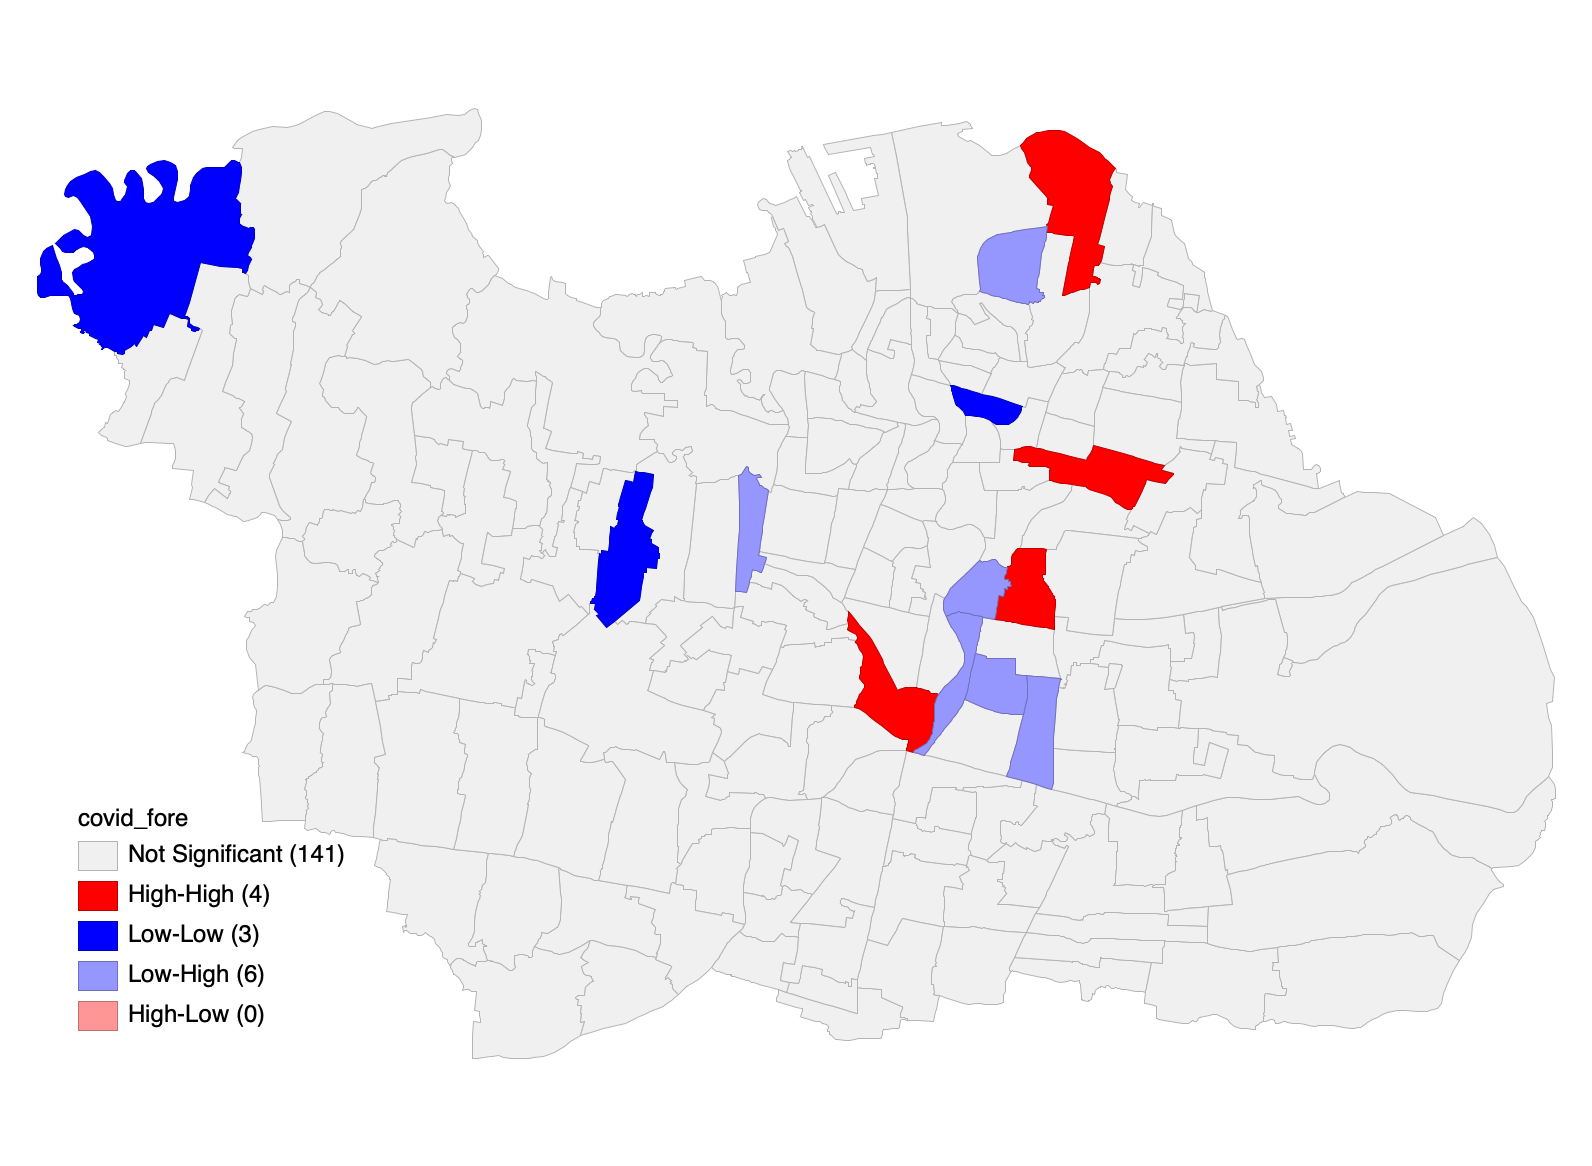
\includegraphics[width=0.49\linewidth]{LocalMoran-CovidBefore} \caption{Local Moran's I Statistics of Electoral Participation and Covid-19 Infection Case}\label{fig:vto}
\end{figure}
\normalsize

~ The maps in Figure 3 show an apparent spatial clustering of voter
turnout in the left-hand map, relative to the cases of Covid-19
infections. With significantly high-high and low-low autocorrelations,
the high voter turnout of 12 villages and the low voter turnout of 33
villages are clustered in the west and in the middle north-east part of
the city, respectively. On the contrary, we do not find spatial
patterning of the Covid-19 infection as massive as that of the electoral
participation.

~ Furthermore, suppose we return to the left-hand map of Figure 1. In
that case, the clustering of the high turnout in the western part of the
city seems to fit the epidemiologist's expectation of the low infection
of the western region, relative to the low turnout in the southern part
of the city. However, the low turnout in the middle north-eastern part
does not meet our low infection expectations. Villages with a low
infection rate are expected to have a cluster of high turnout. This
spatial patterning of turnout leads us to investigate further possible
factors, including proximity of Covid-19 infections, that situate people
to come to polling stations.

\hypertarget{spatial-models-of-turnout}{%
\subsection{Spatial Models of Turnout}\label{spatial-models-of-turnout}}

~ Table 2 reports spatial autoregressive (spatial lag dependence) models
in columns 1-3.\footnote{The spatial models are computed in R where
  GeoDa also reports exactly the same results.}. It also reports the
standard regression (Ordinary Least Square) model in model columns 4-6
to examine the cross-sectional models of turnout. As attached in
Appendix A, theThe Lagrange Multiplier (LM) diagnostics, as attached in
Appendix A, show that both LM for error and lag dependence models are
significant with p-value\textless.05. However, robust LM diagnostics
display that spatial lag model is more statistically significance
(p-value = .1) than the spatial error model (p-value = .5). I report all
the regression statistics for the sake of transparency and
clarification.

~ Though the statistical significance across the models is the same as
those in the standard regression models, the point estimates and
standard errors differ (reduced or corrected) when we specify spatial
parameters into the model. Spatial models assume that observations are
not independent as the interactions occur between units due to their
spatial dimensions. In the models, they are defined as a spatial weight
matrix, i.e., a measure for spatial closeness estimated by sharing
borders.

~ The spatial parameters (\(\rho\)) shown in the Spatial Lag row clearly
suggest that spatial lag dependence occurs in turnout. Across the three
models, the coefficients of the spatial lag are significant (p
\textless{} 0.05) with 0.6065, 0.6098, 0.6003 for the first (crisis
proximity), second (close election), and third (administrative
adjustment) models, respectively. The significant result of the spatial
lag dependence model conforms to the theory of contagious turnout.
Turnout is a result of neighboring effects where effects are a product
of either explicit/implicit social interactions of the diffusion theory
or by external-force mechanisms of the group response theory. Under the
absence of convenient (distance) voting, people who come to vote at the
polling sites are mainly driven by turnout decisions among their
neighbors. This mechanism conforms to the two-dimensional and
multi-directional nature of spatial autocorrelation. Diffusion occurs
when the resulting interactions affect each other across multiple
neighbors.

~ In terms of the cross-sectional OSL models, the results suggest that
Covid-19 proximity in Model 1-2 shows negative coefficients. This result
at a glance follows the theoretical expectation that turnout decreases
when the number of infection cases in the neighborhood is high.
Nevertheless, these estimates are not statistically indistinguishable,
so we are not sure whether voters follow such a theoretical direction.
Political mobilization, approximated by the level of competitiveness
(close election or the margin of votes between candidates), even does
not show any sign of our expectation. This result suggests that pandemic
proximity and political variable do not explain why voters vote (or not)
during the pandemic.

~ More importantly, population size at the polling sites in Model 5-6
clearly explains the voter turnout (p \textless{} .05). Its negative
coefficients in both the original and lagged variables (-0.060) meet the
theoretical expectation that turnout in a large polling site's
population size is low when the population size at the polling site
contributes is relatively large. An increase in population size at the
polling site contributes to a decrease in turnout since people are
cautious when an overcrowded is expected as the result of their
neighboring interactions. But again, this cross-section model is not
sufficient to explain the rise of turnout during the pandemic.

\newpage
\begin{landscape}
\normalsize
\begin{table}[!htbp] \centering 
  \caption{Spatial Autoregressive Models of Voter Turnout$*$} 
  \label{} 
\small 
\begin{tabular}{@{\extracolsep{5pt}}lcccccc} 
\\[-1.8ex]\hline \\[-1.8ex] 
\\[-1.8ex] & \multicolumn{6}{c}{\textbf{Voter Turnout}} \\ 
\\[-1.8ex] & \multicolumn{3}{c}{\textbf{spatial}} & \multicolumn{3}{c}{\textbf{OLS}} \\ 
 & \multicolumn{3}{c}{\textbf{autoregressive}} & \multicolumn{3}{c}{\textbf{}} \\ 
 & \textbf{1} & \textbf{2} & \textbf{3} & \textbf{4} & \textbf{5} & \textbf{6} \\ 
\hline \\[-1.8ex] 
 Covid-19 Proximity & $-$0.092 &  &  & $-$0.117 &  &  \\ 
  & (0.123) &  &  & (0.145) &  &  \\ 
  Competitiveness &  & 0.0002 &  &  & 0.0001 &  \\ 
  &  & (0.0004) &  &  & (0.0005) &  \\ 
  Polling Site's Population &  &  & $-$0.060$^{**}$ &  &  & $-$0.061$^{*}$ \\ 
  &  &  & (0.026) &  &  & (0.031) \\ 
  Income & 4.678$^{*}$ & 4.620$^{*}$ & 4.605$^{*}$ & 6.884$^{**}$ & 6.768$^{**}$ & 6.803$^{**}$ \\ 
  & (2.422) & (2.420) & (2.379) & (2.852) & (2.856) & (2.817) \\ 
  Education & $-$2.883 & $-$3.133 & $-$2.943 & $-$3.046 & $-$3.352 & $-$3.171 \\ 
  & (2.470) & (2.449) & (2.410) & (2.907) & (2.889) & (2.854) \\ 
  Constant & 22.090$^{***}$ & 21.340$^{***}$ & 45.640$^{***}$ & 50.050$^{***}$ & 49.630$^{***}$ & 74.190$^{***}$ \\ 
  & (4.497) & (4.501) & (11.560) & (0.924) & (1.045) & (12.490) \\ 
 Spatial Lag & 0.6065*** & 0.6098*** & 0.6003*** &  &  &  \\ 
N & 152 & 152 & 152 & 152 & 152 & 152 \\ 
R-squared &  &  &  & 0.041 & 0.037 & 0.061 \\ 
Adj. R-squared &  &  &  & 0.021 & 0.017 & 0.042 \\ 
Log Likelihood & $-$463.200 & $-$463.300 & $-$460.900 &  &  &  \\ 
Residual Std. Error (df = 148) &  &  &  & 5.790 & 5.802 & 5.728 \\ 
F Statistic (df = 3; 148) &  &  &  & 2.094 & 1.878 & 3.200$^{**}$ \\ 
Wald Test (df = 1) & 42.640$^{***}$ & 43.540$^{***}$ & 44.450$^{***}$ &  &  &  \\ 
LR Test (df = 1) & 34.710$^{***}$ & 35.120$^{***}$ & 36.060$^{***}$ &  &  &  \\ 
AIC & 938.400 & 938.700 & 933.800 &  &  &  \\ 
\hline \\[-1.8ex] 
\multicolumn{7}{l}{$^{***}$p $<$ .01; $^{**}$p $<$ .05; $^{*}$p $<$ .1} \\ 
\multicolumn{7}{l}{$*$ Obervations are village-level units} \\ 
\end{tabular} 
\end{table} 
\normalsize
\end{landscape}

\hypertarget{discussion}{%
\section{Discussion}\label{discussion}}

~ This paper has shown that electoral participation is not randomly
scattered as the way how people come to vote at the polling sites is
spatially structured. This clustering suggests that turnout is
contagious. Based on the result of the spatial lag model, the contagious
turnout stems from the neighboring effects where social interactions and
group responses occur due to the nature of multi-dimensional and
multi-directional influences of the observations. The result explains
the counterintuitive case as shown in Surabaya and other places where
voter turnout increases in elections held during the pandemic, relative
to those in elections held before the pandemic when convenient voting
procedures (e.g., early, electronic, or postal voting) are even absent.
Voters potentially imitate and influence each other because of their
spatial proximity, reassuring themselves that voting is safe.

~ Though we cannot rely merely on the cross-section models, this paper
also finds that population size is linked to voter turnout at a polling
site. However, political mobilization and Covid-19 proximity do not
explain the electoral behavior. This result suggests that feasible but
simple institutional adjustment of electoral management in a time of
crisis is critical. The voters' cautiousness on the polling site's
population size predicts turnout during the pandemic, rather than the
political competition at the battleground or the proximity of the
Covid-19 infection cases.

~ This study contributes to two broader debates. First, turnout during
pandemic needs to be investigated in the context of crisis. One strategy
is by specifying spatial dimension into the models in order to seek the
neighboring effects on turnout. Distance, location, and other measures
of spatial proximity are essential when people are heavily concerned
with physical measures of the infectious pandemic. Second, it also
contributes to the literature on institutional effects on turnout.
Administrative adjustments still matter in explaining turnout in a time
of Covid-19, rather than a political and direct measure of pandemic
variables. Thus, this study may have policy implications on the way how
elections are held during the pandemic.

~ Nevertheless, it might be premature to suggest that such results are
robust for two reasons. First, the village-level unit of analysis may
not explain social interactions on the ground, compared with, say,
neighboring block-level units (known in Indonesian as \emph{Rukun Warga}
or RW). Second, the models only rely on the key variables. Regarding the
first concern, narrowing down the unit of analysis may help generate
more convincing results due to two reasons. First, a polling site
represents a number of RW-level units where the residents are registered
to vote. So, the assumption of social interactions among individuals
behind the spatial model specifications has an actual basis. Second,
narrowing down into neighboring blocks generates much larger
observations that may also contribute to the law of large numbers in
statistics. RW-level units in Surabaya, for instance, cover more than
1000 blocks where the inhabitants are administratively and spatially
clustered. Therefore, we may have more say to draw and explain the
spatial analyses.

~ Related to the second concern, I wonder whether the lack of necessary
covariates, specifically demographic profiles, is a critical limitation
in this study. Note that the current paper merely employs aggregate
demographic data based on the individual-level study of exit poll survey
which may convey statistical artifact or ecological fallacy. Demographic
variables, or other omitted variables, are most likely to be potential
confounders since demographic characteristics have always been
inevitable variables in explaining voter turnout (Plutzer 2017). The
available data only addresses sub-district demographic profiles, whereas
the village-level demographic characteristics are necessary for model
specification. For instance, level of education and income may affect
the estimates of the effect of the variables of interest. People in
villages with a high level of education or income are arguably more
hesitant to come to the polling station (low turnout) when the proximity
of crisis (Covid-19 infection cases) is high. Thus the next research
agenda is to complement these data types with lower-level units and
include the relevant variables into the model specifications.

\newpage

\hypertarget{references}{%
\section{References}\label{references}}

\hypertarget{refs}{}
\begin{CSLReferences}{1}{0}
\leavevmode\hypertarget{ref-aldrich2017turnout}{}%
Aldrich, John H, and Libby M Jenke. 2017. {``Turnout and the Calculus of
Voting: Recent Advances and Prospects for Integration with Theories of
Campaigns and Elections.''} \emph{The Routledge Handbook of Elections,
Voting Behaviorand Public Opinion}, 83--95.

\leavevmode\hypertarget{ref-aldrich2011turnout}{}%
Aldrich, John H, Jacob M Montgomery, and Wendy Wood. 2011. {``Turnout as
a Habit.''} \emph{Political Behavior} 33 (4): 535--63.

\leavevmode\hypertarget{ref-anselin2007spatial}{}%
Anselin, Luc. 2007. {``Spatial Econometrics.''} In \emph{A Companion to
Theoretical Econometrics}, 310--30. Wiley.

\leavevmode\hypertarget{ref-anselin1995new}{}%
Anselin, Luc, and Raymond JGM Florax. 1995. {``New Directions in Spatial
Econometrics: Introduction.''} In \emph{New Directions in Spatial
Econometrics}, 3--18. Springer.

\leavevmode\hypertarget{ref-asplund2021elections}{}%
Asplund, Lars, Erik, Fakiha Ahmed, Bor Stevense, Sulemana Umar, Toby
James, Alistair Clark, and Peter Wolf. 2021. {``Elections and Covid-19:
How Special Voting Arrangements Were Expanded in 2020.''}
\emph{International IDEA}.

\leavevmode\hypertarget{ref-baller2002social}{}%
Baller, Robert D, and Kelly K Richardson. 2002. {``Social Integration,
Imitation, and the Geographic Patterning of Suicide.''} \emph{American
Sociological Review}, 873--88.

\leavevmode\hypertarget{ref-blais2000vote}{}%
Blais, André. 2000. \emph{To Vote or Not to Vote?: The Merits and Limits
of Rational Choice Theory}. University of Pittsburgh Pre.

\leavevmode\hypertarget{ref-blais1990does}{}%
Blais, André, and R Kenneth Carty. 1990. {``Does Proportional
Representation Foster Voter Turnout?''} \emph{European Journal of
Political Research} 18 (2): 167--81.

\leavevmode\hypertarget{ref-bormann2013democratic}{}%
Bormann, Nils-Christian, and Matt Golder. 2013. {``Democratic Electoral
Systems Around the World, 1946--2011.''} \emph{Electoral Studies} 32
(2): 360--69.

\leavevmode\hypertarget{ref-brady2011turning}{}%
Brady, Henry E, and John E McNulty. 2011. {``Turning Out to Vote: The
Costs of Finding and Getting to the Polling Place.''} \emph{American
Political Science Review} 105 (1): 115--34.

\leavevmode\hypertarget{ref-budi2021does}{}%
Budi, Arya. 2021. {``Does Religious Identity Moderate Economic Voting?
Evidence from Indonesia.''} \emph{Harvard Dataverse} V2.

\leavevmode\hypertarget{ref-cann2011strategic}{}%
Cann, Damon M, and Jeffrey Bryan Cole. 2011. {``Strategic Campaigning,
Closeness, and Voter Mobilization in US Presidential Elections.''}
\emph{Electoral Studies} 30 (2): 344--52.

\leavevmode\hypertarget{ref-cantoni2020precinct}{}%
Cantoni, Enrico. 2020. {``A Precinct Too Far: Turnout and Voting
Costs.''} \emph{American Economic Journal: Applied Economics} 12 (1):
61--85.

\leavevmode\hypertarget{ref-cebula2008impact}{}%
Cebula, Richard J, Garey C Durden, and Patricia E Gaynor. 2008. {``The
Impact of the Repeat-Voting-Habit Persistence Phenomenon on the
Probability of Voting in Presidential Elections.''} \emph{Southern
Economic Journal}, 429--40.

\leavevmode\hypertarget{ref-tam2003contagion}{}%
Cho, Wendy K Tam. 2003. {``Contagion Effects and Ethnic Contribution
Networks.''} \emph{American Journal of Political Science} 47 (2):
368--87.

\leavevmode\hypertarget{ref-tam2011environmental}{}%
Cho, Wendy K Tam, and Neil Baer. 2011. {``Environmental Determinants of
Racial Attitudes Redux: The Critical Decisions Related to
Operationalizing Context.''} \emph{American Politics Research} 39 (2):
414--36.

\leavevmode\hypertarget{ref-cho2010rough}{}%
Cho, Wendy K Tam, and James G Gimpel. 2010. {``Rough Terrain: Spatial
Variation in Campaign Contributing and Volunteerism.''} \emph{American
Journal of Political Science} 54 (1): 74--89.

\leavevmode\hypertarget{ref-cho2008emanating}{}%
Cho, Wendy K Tam, and Thomas J Rudolph. 2008. {``Emanating Political
Participation: Untangling the Spatial Structure Behind Participation.''}
\emph{British Journal of Political Science} 38 (2): 273--89.

\leavevmode\hypertarget{ref-dinas2017acquisition}{}%
Dinas, Elias. 2017. {``The Acquisition of Voting Habits.''} In \emph{The
Routledge Handbook of Elections, Voting Behaviorand Public Opinion},
108--20. Routledge.

\leavevmode\hypertarget{ref-diwakar2008voter}{}%
Diwakar, Rekha. 2008. {``Voter Turnout in the Indian States: An
Empirical Analysis.''} \emph{Journal of Elections, Public Opinion and
Parties} 18 (1): 75--100.

\leavevmode\hypertarget{ref-downs1957economic}{}%
Downs, Anthony. 1957. {``An Economic Theory of Political Action in a
Democracy.''} \emph{The Journal of Political Economy} 65 (2): 135--50.

\leavevmode\hypertarget{ref-dyck2005distance}{}%
Dyck, Joshua J, and James G Gimpel. 2005. {``Distance, Turnout, and the
Convenience of Voting.''} \emph{Social Science Quarterly} 86 (3):
531--48.

\leavevmode\hypertarget{ref-feddersen1999abstention}{}%
Feddersen, Timothy J, and Wolfgang Pesendorfer. 1999. {``Abstention in
Elections with Asymmetric Information and Diverse Preferences.''}
\emph{American Political Science Review} 93 (2): 381--98.

\leavevmode\hypertarget{ref-franklin1999electoral}{}%
Franklin, Mark N. 1999. {``Electoral Engineering and Cross-National
Turnout Differences: What Role for Compulsory Voting?''} \emph{British
Journal of Political Science} 29 (1): 205--16.

\leavevmode\hypertarget{ref-gerber2000effects}{}%
Gerber, Alan S, and Donald P Green. 2000. {``The Effects of Canvassing,
Telephone Calls, and Direct Mail on Voter Turnout: A Field
Experiment.''} \emph{American Political Science Review} 94 (3): 653--63.

\leavevmode\hypertarget{ref-gerber2005correction}{}%
---------. 2005. {``Correction to Gerber and Green (2000), Replication
of Disputed Findings, and Reply to Imai (2005).''} \emph{American
Political Science Review} 99 (2): 301--13.

\leavevmode\hypertarget{ref-gerber2013identifying}{}%
Gerber, Alan S, Gregory A Huber, and Seth J Hill. 2013. {``Identifying
the Effect of All-Mail Elections on Turnout: Staggered Reform in the
Evergreen State.''} \emph{Political Science Research and Methods} 1 (1):
91--116.

\leavevmode\hypertarget{ref-geys2006explaining}{}%
Geys, Benny. 2006. {``Explaining Voter Turnout: A Review of
Aggregate-Level Research.''} \emph{Electoral Studies} 25 (4): 637--63.

\leavevmode\hypertarget{ref-green2019get}{}%
Green, Donald P, and Alan S Gerber. 2019. \emph{Get Out the Vote: How to
Increase Voter Turnout}. Brookings Institution Press.

\leavevmode\hypertarget{ref-grofman1995information}{}%
Grofman, Bernard. 1995. \emph{Information, Participation, and Choice: An
Economic Theory of Democracy in Perspective}. University of Michigan
Press.

\leavevmode\hypertarget{ref-gronke2012voting}{}%
Gronke, Paul, and Peter Miller. 2012. {``Voting by Mail and Turnout in
Oregon: Revisiting Southwell and Burchett.''} \emph{American Politics
Research} 40 (6): 976--97.

\leavevmode\hypertarget{ref-haute2021down}{}%
Haute, Tristan, Camille Kelbel, François Briatte, and Giulia Sandri.
2021. {``Down with Covid: Patterns of Electoral Turnout in the 2020
French Local Elections.''} \emph{Journal of Elections, Public Opinion
and Parties} 31 (sup1): 69--81.

\leavevmode\hypertarget{ref-imai2005get}{}%
Imai, Kosuke. 2005. {``Do Get-Out-the-Vote Calls Reduce Turnout? The
Importance of Statistical Methods for Field Experiments.''}
\emph{American Political Science Review} 99 (2): 283--300.

\leavevmode\hypertarget{ref-indridason2008competition}{}%
Indridason, Indridi H. 2008. {``Competition \& Turnout: The Majority
Run-Off as a Natural Experiment.''} \emph{Electoral Studies} 27 (4):
699--710.

\leavevmode\hypertarget{ref-karp2000going}{}%
Karp, Jeffrey A, and Susan A Banducci. 2000. {``Going Postal: How
All-Mail Elections Influence Turnout.''} \emph{Political Behavior} 22
(3): 223--39.

\leavevmode\hypertarget{ref-kostadinova2007does}{}%
Kostadinova, Tatiana, and Timothy J Power. 2007. {``Does Democratization
Depress Participation? Voter Turnout in the Latin American and Eastern
European Transitional Democracies.''} \emph{Political Research
Quarterly} 60 (3): 363--77.

\leavevmode\hypertarget{ref-merkley2022communicating}{}%
Merkley, Eric, Thomas Bergeron, Peter John Loewen, Angelo Elias, and
Miriam Lapp. 2022. {``Communicating Safety Precautions Can Help Maintain
in-Person Voter Turnout During a Pandemic.''} \emph{Electoral Studies}
75: 102421.

\leavevmode\hypertarget{ref-morton2015exit}{}%
Morton, Rebecca B, Daniel Muller, Lionel Page, and Benno Torgler. 2015.
{``Exit Polls, Turnout, and Bandwagon Voting: Evidence from a Natural
Experiment.''} \emph{European Economic Review} 77: 65--81.

\leavevmode\hypertarget{ref-noury2021does}{}%
Noury, Abdul, Abel François, Olivier Gergaud, and Alexandre Garel. 2021.
{``How Does COVID-19 Affect Electoral Participation? Evidence from the
French Municipal Elections.''} \emph{PloS One} 16 (2): e0247026.

\leavevmode\hypertarget{ref-nwankwo2021covid}{}%
Nwankwo, Cletus Famous. 2021. {``COVID-19 Pandemic and Political
Participation in Lagos, Nigeria.''} \emph{SN Social Sciences} 1 (6):
1--23.

\leavevmode\hypertarget{ref-orford2011changes}{}%
Orford, Scott, Colin Railings, Michael Thrasher, and Galina Borisyuk.
2011. {``Changes in the Probability of Voter Turnout When Resiting
Polling Stations: A Case Study in Brent, UK.''} \emph{Environment and
Planning C: Government and Policy} 29 (1): 149--69.

\leavevmode\hypertarget{ref-pettigrew2021downstream}{}%
Pettigrew, Stephen. 2021. {``The Downstream Consequences of Long Waits:
How Lines at the Precinct Depress Future Turnout.''} \emph{Electoral
Studies} 71: 102188.

\leavevmode\hypertarget{ref-plutzer2017demographics}{}%
Plutzer, Eric. 2017. {``Demographics and the Social Bases of Voter
Turnout.''} In \emph{The Routledge Handbook of Elections, Voting
Behaviorand Public Opinion}, 69--82. Routledge.

\leavevmode\hypertarget{ref-richey2008voting}{}%
Richey, Sean. 2008. {``Voting by Mail: Turnout and Institutional Reform
in Oregon.''} \emph{Social Science Quarterly} 89 (4): 902--15.

\leavevmode\hypertarget{ref-rosenstone1993mobilization}{}%
Rosenstone, Steven J, and John Mark Hansen. 1993. \emph{Mobilization,
Participation, and Democracy in America}. Longman Publishing Group.

\leavevmode\hypertarget{ref-schur2017disability}{}%
Schur, Lisa, Mason Ameri, and Meera Adya. 2017. {``Disability, Voter
Turnout, and Polling Place Accessibility.''} \emph{Social Science
Quarterly} 98 (5): 1374--90.

\leavevmode\hypertarget{ref-simonovits2012competition}{}%
Simonovits, Gábor. 2012. {``Competition and Turnout Revisited: The
Importance of Measuring Expected Closeness Accurately.''}
\emph{Electoral Studies} 31 (2): 364--71.

\leavevmode\hypertarget{ref-soedarsono2020family}{}%
Soedarsono, Soedarsono. 2020. {``A Family Cluster of Coronavirus Disease
(COVID-19) Infection with Different Clinical Manifestations.''}
\emph{Acta Medica Indonesiana} 52 (2): 155--62.

\leavevmode\hypertarget{ref-southwell2000effect}{}%
Southwell, Priscilla L, and Justin I Burchett. 2000. {``The Effect of
All-Mail Elections on Voter Turnout.''} \emph{American Politics
Quarterly} 28 (1): 72--79.

\leavevmode\hypertarget{ref-stockemer2017affects}{}%
Stockemer, Daniel. 2017. {``What Affects Voter Turnout? A Review
Article/Meta-Analysis of Aggregate Research.''} \emph{Government and
Opposition} 52 (4): 698--722.

\leavevmode\hypertarget{ref-voss2006county}{}%
Voss, Paul R, David D Long, Roger B Hammer, and Samantha Friedman. 2006.
{``County Child Poverty Rates in the US: A Spatial Regression
Approach.''} \emph{Population Research and Policy Review} 25 (4):
369--91.

\leavevmode\hypertarget{ref-vowles2017big}{}%
Vowles, Jack. 2017. {``The Big Picture: Turnout at the Macro-Level.''}
In \emph{The Routledge Handbook of Elections, Voting Behaviorand Public
Opinion}, 57--68. Routledge.

\end{CSLReferences}

\newpage

\hypertarget{appendix-a-lagrange-multiplier-diagnostics}{%
\section{Appendix A: Lagrange Multiplier
Diagnostics}\label{appendix-a-lagrange-multiplier-diagnostics}}

\normalsize

Lagrange multiplier diagnostics for spatial dependence

data:\\
model: lm(formula = prcvto \textasciitilde{} coviddiff + incomepr +
edupr, data = dat) weights: datweight

LMerr = 45, df = 1, p-value = 0.00000000002

\begin{verbatim}
Lagrange multiplier diagnostics for spatial dependence
\end{verbatim}

data:\\
model: lm(formula = prcvto \textasciitilde{} coviddiff + incomepr +
edupr, data = dat) weights: datweight

RLMerr = 0.4, df = 1, p-value = 0.5

\begin{verbatim}
Lagrange multiplier diagnostics for spatial dependence
\end{verbatim}

data:\\
model: lm(formula = prcvto \textasciitilde{} coviddiff + incomepr +
edupr, data = dat) weights: datweight

LMlag = 47, df = 1, p-value = 7e-12

\begin{verbatim}
Lagrange multiplier diagnostics for spatial dependence
\end{verbatim}

data:\\
model: lm(formula = prcvto \textasciitilde{} coviddiff + incomepr +
edupr, data = dat) weights: datweight

RLMlag = 2.6, df = 1, p-value = 0.1

\normalsize

\end{document}
